\documentclass[conference]{IEEEtran}
\IEEEoverridecommandlockouts

\usepackage{cite}
\usepackage{amsmath,amssymb}
\usepackage{graphicx}
\usepackage{booktabs}
\usepackage{array}
\usepackage{tikz}
\usetikzlibrary{positioning,arrows.meta,fit}
\usepackage[hidelinks]{hyperref}

\begin{document}

\title{Vetra: Offline AI-Based Health Monitoring and Early Disease Diagnosis for Farm Animals}

% TODO: replace the placeholders below with your team, department and institution.
\author{\IEEEauthorblockN{Aayush Kumar}
\IEEEauthorblockA{\textit{Department of [Department Name]} \\
\textit{[Institution Name]}\\
{[City]}, India \\
{[email address]}}
}

\maketitle

\begin{abstract}
Livestock disease is often noticed only once an animal is visibly ill, by which
point treatment is costlier and infection may already have spread. This paper
presents Vetra, a software system for continuous health monitoring and early
diagnosis of farm animals that runs fully offline. Physiological and behavioural
signals---heart rate, body temperature, respiratory rate, SpO\textsubscript{2},
activity, rumination and gait---are grouped into one-hour windows, converted into
69 features, and classified into eight conditions by a compact neural network
alongside rule-based clinical checks. An alert policy turns per-window
predictions into a small number of actionable alerts, and records are stored
locally and synchronised to a cloud dashboard when connectivity is available.
Evaluated on 48 animals never seen during training, the neural network achieves
a macro-F1 score of 0.981 with a model size of 12.2\,KB, and the alert policy
reduces alert volume by 99.2\% while detecting all 35 sick animals and raising
no alerts for the 13 healthy ones. Because the training data is simulated from
published veterinary reference ranges, these results validate the pipeline
rather than clinical performance.
\end{abstract}

\begin{IEEEkeywords}
precision livestock farming, animal health monitoring, disease diagnosis,
edge AI, TensorFlow Lite, alert fatigue, offline inference
\end{IEEEkeywords}

\section{Introduction}
Livestock is a major source of income for smallholder farmers in India, and an
undetected illness in a single animal can mean lost milk yield, treatment costs
or the spread of infection through a herd. In practice, disease is usually
noticed by eye, once an animal stops eating or moving normally---well after the
physiological signs first appeared.

Continuous monitoring can shift detection earlier. Changes in temperature,
heart rate, breathing and rumination often precede visible symptoms
\cite{neethirajan2017}, and precision livestock farming has made the case for
using such signals to manage individual animals rather than whole herds
\cite{berckmans2017}. Two practical obstacles remain for rural deployment.
First, internet connectivity is intermittent, so a system that sends data to a
server for diagnosis stops working when the link drops. Second, a system that
raises an alert for every abnormal reading quickly overwhelms the farmer and is
ignored.

Vetra addresses both. Every diagnosis is made locally with a model small enough
for low-cost devices, and the cloud is used only to store and display records.
A dedicated alert policy is treated as a core component, not an afterthought.
The project is implemented entirely in software; animal vital signs are
generated by a simulator built on published veterinary reference values.

The objectives of the project are:
\begin{enumerate}
\item A data acquisition and processing pipeline for animal vital signs.
\item Machine learning models that predict disease from those signals.
\item A lightweight model that runs without internet access.
\item Intelligent alert generation that limits false and repeated alerts.
\item Health record storage with cloud synchronisation.
\item A dashboard for farmers and veterinarians.
\end{enumerate}

\section{Related Work}
Wearable sensors for livestock now measure temperature, activity, rumination
and location, and have been reviewed extensively as tools for early disease
detection \cite{neethirajan2017}. Precision livestock farming frames these
sensors as part of a control loop in which each animal is monitored and managed
individually \cite{berckmans2017}. Edge computing moves computation close to the
data source, reducing dependence on network links and lowering latency
\cite{shi2016edge}; quantisation techniques make neural network inference
practical on such constrained hardware \cite{jacob2018quant}.

Vetra combines these ideas into a single pipeline aimed at intermittently
connected farms, and adds an explicit, measured alert policy, since alert volume
largely decides whether such a system is used in practice.

\section{System Architecture}
Fig.~\ref{fig:arch} shows the system. It has three tiers: a local gateway that
performs all diagnosis, a cloud service that stores records, and a web
dashboard.

\begin{figure}[t]
\centering
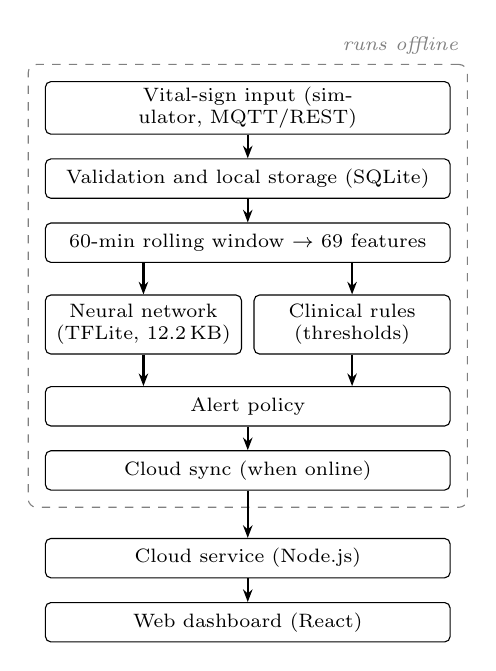
\begin{tikzpicture}[
  node distance=0.3cm,
  box/.style={draw, rounded corners=2pt, align=center, font=\scriptsize,
              text width=5.0cm, minimum height=0.5cm, inner sep=2pt},
  half/.style={draw, rounded corners=2pt, align=center, font=\scriptsize,
              text width=2.35cm, minimum height=0.75cm, inner sep=2pt},
  arr/.style={-{Stealth[length=1.6mm]}, thick}]
\node[box] (sim) {Vital-sign input (simulator, MQTT/REST)};
\node[box, below=of sim] (val) {Validation and local storage (SQLite)};
\node[box, below=of val] (win) {60-min rolling window $\rightarrow$ 69 features};
\node[half, below=0.4cm of win.south west, anchor=north west] (nn) {Neural network\\(TFLite, 12.2\,KB)};
\node[half, below=0.4cm of win.south east, anchor=north east] (rules) {Clinical rules\\(thresholds)};
\node[box, below=0.4cm of nn.south west, anchor=north west] (alert) {Alert policy};
\node[box, below=of alert] (sync) {Cloud sync (when online)};
\node[draw, dashed, gray, rounded corners=3pt, inner sep=6pt,
      fit=(sim) (val) (win) (nn) (rules) (alert) (sync)] (edge) {};
\node[font=\scriptsize\itshape, gray, anchor=south east] at (edge.north east) {runs offline};
\node[box, below=0.6cm of sync] (cloud) {Cloud service (Node.js)};
\node[box, below=of cloud] (dash) {Web dashboard (React)};
\draw[arr] (sim) -- (val);
\draw[arr] (val) -- (win);
\draw[arr] (win.south -| nn) -- (nn);
\draw[arr] (win.south -| rules) -- (rules);
\draw[arr] (nn) -- (alert.north -| nn);
\draw[arr] (rules) -- (alert.north -| rules);
\draw[arr] (alert) -- (sync);
\draw[arr] (sync) -- (cloud);
\draw[arr] (cloud) -- (dash);
\end{tikzpicture}
\caption{Vetra architecture. Everything inside the dashed box runs without an
internet connection.}
\label{fig:arch}
\end{figure}

\subsection{Local gateway}
The gateway receives readings over MQTT \cite{mqtt311} or REST, validates them
against plausible physiological ranges, and stores them in a local SQLite
database. For each animal it keeps a rolling 60-minute window; every 30 minutes
it computes features, runs the model and the clinical rules, and passes the
result to the alert policy. If the network is unavailable, monitoring continues
and records accumulate locally.

\subsection{Cloud service and dashboard}
A Node.js service receives synchronised animals, telemetry, diagnoses and alerts,
stores them as health records, and pushes updates to a React dashboard using
server-sent events. The dashboard shows the herd, per-animal vital-sign charts
and open alerts, which a user can acknowledge.

\subsection{Synchronisation}
Each local table carries a nullable \texttt{synced\_at} column instead of a
separate outbox. Rows are marked synced only after the server acknowledges
them, so an interrupted upload is simply retried and no record is lost. Tables
are uploaded in dependency order---animals, telemetry, diagnoses, alerts.

\section{Methodology}

\subsection{Data generation}
No public dataset of continuous, labelled, multi-channel vital signs for Indian
livestock was available. Vetra therefore simulates a herd of 240 animals over
five days at one reading per minute, covering cattle, buffalo, goats and sheep.
Resting ranges for each species are taken from standard veterinary references
\cite{merck,jackson2002}; for example, cattle are modelled with a heart rate of
48--84\,bpm and a rectal temperature of 38.0--39.3\,\textdegree C. Heat load is
modelled with the temperature--humidity index (THI) \cite{nrc1971}:
\begin{equation}
\mathrm{THI} = 0.8\,T + \frac{RH}{100}\,(T - 14.4) + 46.4,
\end{equation}
where $T$ is air temperature in \textdegree C and $RH$ is relative humidity in
percent.

Each disease is encoded as the change it produces in each signal at full
severity (Table~\ref{tab:conditions}). Acute conditions ramp up from an onset
time over 6--36 hours; chronic ones (obesity, diabetes) are present from the
start. A window is labelled diseased only once mean severity exceeds 0.15, so
the model is not trained to find illness in noise.

\begin{table}[t]
\caption{Simulated Conditions and Their Distinguishing Signs}
\label{tab:conditions}
\centering
\footnotesize
\begin{tabular}{@{}p{2.55cm}>{\raggedright\arraybackslash}p{5.15cm}@{}}
\toprule
\textbf{Condition} & \textbf{Distinguishing sign} \\
\midrule
Cardiac disorder & Heart rate stays high at rest; irregular rhythm \\
Respiratory disease & Faster breathing with falling SpO\textsubscript{2} \\
Obesity & Chronic inactivity; no fever; normal gait \\
Diabetes & High variance in activity rather than a shifted mean \\
Heat stress & Panting under high THI; SpO\textsubscript{2} near normal \\
Infectious disease & Fever with preserved SpO\textsubscript{2} \\
Mobility disorder & Irregular gait with normal temperature \\
\bottomrule
\end{tabular}
\end{table}

\subsection{Feature extraction}
Readings are grouped into 60-minute windows with 50\% overlap. Each window
yields 69 features of two kinds. Species-normalised absolute values detect
conditions already present when monitoring begins, such as obesity. Deviations
from the animal's own trailing 24-hour baseline detect acute change, such as
fever; the baseline is shifted by one sample so a window never contributes to
the baseline it is compared against. The same feature function is used during
training and on the gateway, and a test checks that both paths produce
identical output.

\subsection{Train--test split}
Because overlapping windows from one animal are nearly identical, a random split
would place almost the same rows in both training and test sets and inflate
every metric. The data is therefore split by animal: 20\% of animals are held
out for testing and 15\% of the remainder for validation, with no animal in
more than one set. All results are reported on the 48 held-out test animals
(11{,}472 windows).

\subsection{Models}
Three classical baselines were trained with scikit-learn \cite{pedregosa2011}:
multinomial logistic regression, a random forest \cite{breiman2001} with 300
trees, and histogram gradient boosting \cite{friedman2001}. The deployed model
is a compact neural network built in TensorFlow \cite{abadi2016}: a
normalisation layer, dense layers of 64 and 32 ReLU units with dropout of 0.2
and 0.1, and an eight-class softmax output. It is trained with Adam
\cite{kingma2015} (learning rate $10^{-3}$, batch size 256, up to 80 epochs) with
class weighting and early stopping on validation loss.

\subsection{Edge model export}
The network is converted to TensorFlow Lite in three variants: float32,
dynamic-range int8 and full int8 \cite{jacob2018quant}. Each variant is compared
with the float model on the test set, and any variant that disagrees on more
than 1\% of predictions is rejected automatically. The normalisation layer is
kept inside the exported model, so no separate scaler file has to be kept in
step with it.

\subsection{Clinical rules}
Rule-based checks run alongside the model and fire on textbook thresholds
regardless of its prediction---for example fever, resting tachycardia, low
SpO\textsubscript{2}, a sharp drop in rumination against the animal's
baseline, and THI above 78, 84 or 88. The rules give the veterinarian a readable
reason (``SpO\textsubscript{2} 88\%, respiratory rate 64/min'') rather than a
bare probability, and ensure a critical sign is never missed because of a model
error.

\subsection{Alert policy}
Raising an alert for every abnormal window would produce about 26 alerts per
animal per day. The policy instead requires:
\begin{itemize}
\item \textbf{Confirmation:} two matching windows out of the last four, each with
confidence of at least 0.60.
\item \textbf{Hysteresis:} three consecutive healthy windows before an alert is
resolved.
\item \textbf{Cooldown:} six hours before the same condition can re-alert.
\item \textbf{Deduplication:} at most one open alert per animal per condition.
\end{itemize}
A critical clinical rule bypasses confirmation and alerts immediately.

\section{Results}

\subsection{Diagnosis}
Table~\ref{tab:diag} compares the best classical baseline, logistic regression,
with the deployed neural network on the held-out animals, and
Table~\ref{tab:perclass} gives the network's per-class scores. Diabetes has the
lowest recall (0.921); most of its errors are windows classified as healthy,
which is expected since it is defined by activity variance rather than a clear
shift in any one signal.

\begin{table}[t]
\caption{Diagnosis Performance on Held-Out Animals}
\label{tab:diag}
\centering
\footnotesize
\begin{tabular}{@{}lcc@{}}
\toprule
\textbf{Metric} & \textbf{Logistic regression} & \textbf{Neural network} \\
\midrule
Macro-F1 & 0.986 & 0.981 \\
Screening recall & 0.985 & 0.977 \\
False-alarm rate & 0.008 & 0.009 \\
Model size & 7\,KB & 12.2\,KB \\
\bottomrule
\end{tabular}
\end{table}

\begin{table}[t]
\caption{Neural Network Per-Class Performance}
\label{tab:perclass}
\centering
\footnotesize
\begin{tabular}{@{}lcccr@{}}
\toprule
\textbf{Class} & \textbf{Precision} & \textbf{Recall} & \textbf{F1} & \textbf{Windows} \\
\midrule
Healthy & 0.972 & 0.991 & 0.982 & 5{,}177 \\
Cardiac disorder & 0.982 & 0.992 & 0.987 & 611 \\
Respiratory disease & 0.946 & 1.000 & 0.972 & 369 \\
Obesity & 0.997 & 0.993 & 0.995 & 1{,}434 \\
Diabetes & 0.993 & 0.921 & 0.955 & 1{,}673 \\
Heat stress & 0.988 & 0.975 & 0.981 & 670 \\
Infectious disease & 0.990 & 0.986 & 0.988 & 707 \\
Mobility disorder & 0.982 & 0.999 & 0.991 & 831 \\
\bottomrule
\end{tabular}
\end{table}

Since the aim is early detection, recall was also measured by disease severity
(Table~\ref{tab:severity}). Early-stage cases are the hardest, at 88.4\% recall,
with recall above 96\% at later stages.

\begin{table}[t]
\caption{Neural Network Recall by Disease Severity}
\label{tab:severity}
\centering
\footnotesize
\begin{tabular}{@{}lcc@{}}
\toprule
\textbf{Severity band} & \textbf{Severity range} & \textbf{Recall} \\
\midrule
Early & 0.15--0.35 & 0.884 \\
Mild & 0.35--0.55 & 0.993 \\
Marked & 0.55--0.75 & 0.967 \\
Severe & 0.75--1.00 & 0.984 \\
\bottomrule
\end{tabular}
\end{table}

\subsection{Edge deployment}
Table~\ref{tab:tflite} lists the exported variants. Full-int8 quantisation
agreed with the float model on only 46\% of predictions and fell to 0.08
macro-F1, because the raw features span very different scales (from about 0.9
to several thousand) and an 8-bit input cannot represent both. The agreement
check rejected it automatically, and the dynamic-range int8 model was selected.
The full streaming pipeline (validation, windowing, feature extraction and
inference) processes about 5{,}000 readings per second on a single core of a
development laptop.

\begin{table}[t]
\caption{TensorFlow Lite Variants}
\label{tab:tflite}
\centering
\footnotesize
\begin{tabular}{@{}lcccc@{}}
\toprule
\textbf{Variant} & \textbf{Size} & \textbf{Agreement} & \textbf{Latency} & \textbf{Status} \\
\midrule
float32 & 29.9\,KB & 1.0000 & 0.0066\,ms & -- \\
Dynamic int8 & 12.2\,KB & 0.9997 & 0.0064\,ms & Selected \\
Full int8 & 13.0\,KB & 0.4599 & 0.0076\,ms & Rejected \\
\bottomrule
\end{tabular}
\end{table}

\subsection{Alerts}
The alert policy was evaluated on the 48 held-out animals over 240 animal-days
(Table~\ref{tab:alerts}). It reduces alert volume by 99.2\% without missing any
sick animal, and the median delay from disease onset to alert is 1.5 hours.

\begin{table}[t]
\caption{Alert Policy Evaluation (48 Animals, 240 Animal-Days)}
\label{tab:alerts}
\centering
\footnotesize
\begin{tabular}{@{}lcc@{}}
\toprule
\textbf{Measure} & \textbf{Every abnormal window} & \textbf{With policy} \\
\midrule
Alerts raised & 6{,}200 & 52 \\
Alerts per animal-day & 25.83 & 0.22 \\
Sick animals detected & 35/35 & 35/35 \\
Healthy animals alerted & -- & 0/13 \\
Median time from onset & -- & 1.5\,h \\
\bottomrule
\end{tabular}
\end{table}

\subsection{Testing}
The system is covered by 70 Python tests and 20 Node.js API tests, all passing.
They include checks that no animal appears in two data splits, that training
and streaming features are identical, and that the alert policy, rules and
local store behave as specified.

\section{Discussion and Limitations}
The main limitation is that the data is simulated. The results therefore show
that the pipeline is sound---the split does not leak, the features carry the
signal, the model fits in 12.2\,KB and runs offline, and the alert policy
suppresses noise without losing sick animals---but they do not measure clinical
accuracy. That a logistic regression scores 0.986 suggests the simulated disease
signatures are cleaner than real presentations; on real data all metrics would
be expected to fall, with non-linear models likely pulling ahead.

Real animals also present with multiple simultaneous conditions, missing sensor
readings and diseases outside the eight modelled classes. The design limits the
cost of moving to real data: only the data generator needs to be replaced by a
loader producing the same columns.

The current security model is minimal: a shared API key protects
synchronisation, and the dashboard has no user accounts. A production
deployment would need per-gateway credentials, authenticated sessions and
encrypted connections.

\section{Conclusion and Future Work}
Vetra demonstrates an end-to-end, offline-capable pipeline for livestock health
monitoring: from vital signs through feature extraction, a 12.2\,KB diagnostic
model and clinical rules, to an alert policy that cuts alert volume by 99.2\%
while detecting every sick animal in the test herd.

Planned work includes:
\begin{itemize}
\item \textbf{Symptom-selection interface:} a form where the user selects an
animal's symptoms or readings from drop-down lists and receives a diagnosis,
confidence level and recommended action.
\item \textbf{Veterinarian feedback:} recording confirmed diagnoses against each
alert, building a real labelled dataset for retraining.
\item \textbf{Farmer notifications:} SMS or WhatsApp alerts in local languages.
\item \textbf{Outbreak detection:} flagging clusters of nearby animals that show
infectious signs within a short period.
\end{itemize}

\begin{thebibliography}{00}
\bibitem{neethirajan2017} S. Neethirajan, ``Recent advances in wearable sensors
for animal health management,'' \textit{Sens. Bio-Sens. Res.}, vol.~12,
pp.~15--29, 2017.
\bibitem{berckmans2017} D. Berckmans, ``General introduction to precision
livestock farming,'' \textit{Anim. Front.}, vol.~7, no.~1, pp.~6--11, 2017.
\bibitem{shi2016edge} W. Shi, J. Cao, Q. Zhang, Y. Li, and L. Xu, ``Edge
computing: Vision and challenges,'' \textit{IEEE Internet Things J.}, vol.~3,
no.~5, pp.~637--646, Oct. 2016.
\bibitem{jacob2018quant} B. Jacob \textit{et al.}, ``Quantization and training
of neural networks for efficient integer-arithmetic-only inference,'' in
\textit{Proc. IEEE Conf. Comput. Vis. Pattern Recognit. (CVPR)}, 2018,
pp.~2704--2713.
\bibitem{mqtt311} OASIS, ``MQTT Version 3.1.1,'' OASIS Standard, Oct. 2014.
\bibitem{merck} \textit{MSD Veterinary Manual}. Rahway, NJ, USA: Merck \& Co.
[Online]. Available: https://www.msdvetmanual.com
\bibitem{jackson2002} P. G. G. Jackson and P. D. Cockcroft, \textit{Clinical
Examination of Farm Animals}. Oxford, U.K.: Blackwell Science, 2002.
\bibitem{nrc1971} National Research Council, \textit{A Guide to Environmental
Research on Animals}. Washington, DC, USA: Nat. Acad. Sci., 1971.
\bibitem{pedregosa2011} F. Pedregosa \textit{et al.}, ``Scikit-learn: Machine
learning in Python,'' \textit{J. Mach. Learn. Res.}, vol.~12, pp.~2825--2830,
2011.
\bibitem{breiman2001} L. Breiman, ``Random forests,'' \textit{Mach. Learn.},
vol.~45, no.~1, pp.~5--32, 2001.
\bibitem{friedman2001} J. H. Friedman, ``Greedy function approximation: A
gradient boosting machine,'' \textit{Ann. Statist.}, vol.~29, no.~5,
pp.~1189--1232, 2001.
\bibitem{abadi2016} M. Abadi \textit{et al.}, ``TensorFlow: A system for
large-scale machine learning,'' in \textit{Proc. 12th USENIX Symp. Oper. Syst.
Des. Implement. (OSDI)}, 2016, pp.~265--283.
\bibitem{kingma2015} D. P. Kingma and J. Ba, ``Adam: A method for stochastic
optimization,'' in \textit{Proc. Int. Conf. Learn. Represent. (ICLR)}, 2015.
\end{thebibliography}

\end{document}
